\section{Results}
\label{sec:results}

All numbers are at $\alpha=0.1$ unless stated. Coverage statistics over
subjects are computed by merging per-subject coverage across the five folds
and averaging it over the seeds and backbones that re-run the same
partition, so each subject appears exactly once; the spread reported is the
run-to-run spread of the training, not a spread over patient cohorts.

\paragraph{Backbone performance}
\Cref{tab:training} reports classification quality. Both backbones sit in the
range published for Sleep-EDF on Fpz--Cz, with \texttt{sleepcnn} slightly
ahead of \texttt{eegnet} on accuracy and kappa. N1 remains the weak class for
both, and the per-stage breakdown in \Cref{tab:perclass} shows that the
marginal number hides class-level deviations in both directions. ECE is modest ($0.030$ for \texttt{eegnet}), and
\Cref{sec:results-patient} shows that this is precisely the number that fails
to detect the problem: a well-calibrated marginal predictor can still leave a
patient twelve points short of nominal coverage.

\begin{table}[t]
\centering
\small
\setlength{\tabcolsep}{4pt}
\caption{Backbone classification performance on the test subjects, over all folds and seeds (mean $\pm$ standard deviation).}
\label{tab:training}
\resizebox{\ifdim\width>\linewidth \linewidth\else\width\fi}{!}{%
\begin{tabular}{lrrrrr}
\toprule
Model & Accuracy & Cohen's $\kappa$ & Macro-F1 & ECE & Runs \\
\midrule
\texttt{eegnet} & 0.781 $\pm$ 0.042 & 0.698 $\pm$ 0.058 & 0.644 $\pm$ 0.034 & 0.030 $\pm$ 0.013 & 15 \\
\texttt{sleepcnn} & 0.803 $\pm$ 0.042 & 0.728 $\pm$ 0.058 & 0.711 $\pm$ 0.043 & 0.032 $\pm$ 0.017 & 15 \\
\bottomrule
\end{tabular}}
\end{table}


\subsection{The marginal guarantee is not the patient guarantee}
\label{sec:results-patient}

\Cref{tab:sacp} contrasts pooled calibration with the patient-level
statistics. Pooled APS reaches $0.898$ marginal coverage --- nominal to within
two thousandths --- while the worst patient is covered at $0.774$, $45\%$ of
the patients fall below $1-\alpha$, and per-patient coverage has a standard
deviation of $0.051$. The quantity that matters clinically is the
\emph{patient coverage gap},
\begin{equation}
\max_{j}\big[(1-\alpha)-\mathrm{cov}_j\big]^{+},
\end{equation}
and it is invisible in the marginal number. The first row makes the point sharper: a random-epoch split --- the
protocol under which subjects are mixed between calibration and test ---
reports $0.901$ coverage. A per-patient figure could be computed there ---
epochs carry their subject identifier --- but it would measure the epochs
shared between calibration and test rather than the subject, so the row is
reported with marginal coverage and set size only. The split that makes the
statistic estimable is the same split that makes the failure visible.

The class-conditional (Mondrian) row is the informative baseline, and it
deserves care because it is not a straw man. Conditioning the threshold on the
stage makes the mean set \emph{smaller} --- from $2.54$ to $2.29$ labels per
epoch --- because a per-class APS threshold no longer has to pay for the heavy
tail of the pooled score, and it nudges the patient statistics in the right
direction: worst-patient coverage rises from $0.774$ to $0.787$ and the
per-patient standard deviation falls from $0.051$ to $0.048$. The nudges are
small, and a paired per-patient test on the distance from nominal finds no
difference from pooled calibration (smaller for $12$ of $20$ patients,
$p=0.43$). The mechanism is that patient difficulty is strongly associated with
stage mix --- every patient is hard on N1 --- so a stage-conditional rule
equalises patients only to the extent that they differ by stage alone. What it
cannot do is adapt to a patient who is hard for reasons orthogonal to their
stage mix, and on this cohort it still leaves an $0.11$ gap at the worst
patient and $45\%$ of patients below nominal. The same limitation applies to
the per-stage threshold on the deficit score of \Cref{sec:results-score}:
conditioning reaches a patient only through their stage mix, so it reduces
the fraction of patients below nominal from $0.60$ to $0.35$ but leaves the
worst patient where it was ($0.787$ against $0.792$). That residual is the
target of \Cref{sec:results-aci}.

\begin{table}[t]
\centering
\small
\setlength{\tabcolsep}{4pt}
\caption{Coverage over patients at $\alpha=0.1$. Per-subject coverage is merged across the five subject-wise folds, so each of the 20 subjects appears exactly once. The random-epoch row is the protocol that mixes epochs from all subjects between calibration and test; a per-patient decomposition under it would measure the shared epochs rather than the subject, so the row reports marginal coverage and set size only.}
\label{tab:sacp}
\resizebox{\ifdim\width>\linewidth \linewidth\else\width\fi}{!}{%
\begin{tabular}{lrrrrrrr}
\toprule
Method & Coverage & Worst subj. & $p_{10}$ subj. & SD & Below & Set size & Singleton \\
\midrule
Random-epoch split & 0.901 & -- & -- & -- & -- & 2.542 & -- \\
Pooled (APS) & 0.898 $\pm$ 0.038 & 0.774 & 0.822 & 0.0510 & 0.45 & 2.537 $\pm$ 0.207 & 0.167 $\pm$ 0.051 \\
Pooled (RAPS) & 0.885 $\pm$ 0.037 & 0.785 & 0.836 & 0.0397 & 0.65 & 1.614 $\pm$ 0.206 & 0.472 $\pm$ 0.178 \\
Mondrian (per class) & 0.896 $\pm$ 0.031 & 0.787 & 0.835 & 0.0480 & 0.45 & 2.294 $\pm$ 0.157 & 0.230 $\pm$ 0.062 \\
$k$NN subject (APS) & 0.894 $\pm$ 0.040 & 0.759 & 0.828 & 0.0536 & 0.50 & 2.509 $\pm$ 0.214 & 0.170 $\pm$ 0.049 \\
Warm-up SACP, $m=80$ & 0.897 $\pm$ 0.036 & 0.782 & 0.820 & 0.0496 & 0.40 & 2.552 $\pm$ 0.299 & 0.172 $\pm$ 0.055 \\
Warm-up SACP, $m=320$ & 0.891 $\pm$ 0.031 & 0.769 & 0.829 & 0.0516 & 0.50 & 2.519 $\pm$ 0.151 & 0.155 $\pm$ 0.045 \\
Oracle per patient & 0.901 $\pm$ 0.000 & 0.901 & 0.901 & 0.0004 & 0.00 & 2.492 $\pm$ 0.230 & 0.180 $\pm$ 0.058 \\
Per-patient ACI (APS) & 0.904 $\pm$ 0.010 & 0.886 & 0.892 & 0.0117 & 0.50 & 2.491 $\pm$ 0.203 & 0.177 $\pm$ 0.060 \\
Per-patient ACI (deficit) & 0.898 $\pm$ 0.007 & 0.872 & 0.891 & 0.0097 & 0.70 & 1.575 $\pm$ 0.271 & 0.831 $\pm$ 0.072 \\
\bottomrule
\end{tabular}}
\par\vspace{2pt}{\footnotesize ``Coverage'' is marginal over epochs (mean $\pm$ SD over the runs); ``Worst subj.'' is the minimum per-subject coverage over the runs; ``Below'' is the fraction of subjects below $1-\alpha$; ``SD'' is the standard deviation of per-subject coverage. Each subject contributes one value per run, the runs being five folds $\times$ three seeds $\times$ two backbones; set size and singleton rate are averaged over the same runs.}
\end{table}


\subsection{Posterior smoothing is the largest efficiency lever}
\label{sec:results-score}

\Cref{tab:temporal} compares nonconformity scores on the same epochs and the
same calibration data. Replacing the raw-softmax APS score with the smoothed
posterior deficit reduces the mean set size from $2.54$ to $1.53$ labels per
epoch at essentially the same coverage ($0.898$ against $0.889$, a difference
within the run spread), and raises the Jaccard consistency statistic from
$0.68$ to $0.94$. Both sit close to nominal --- the deficit score $1.1$ points
below and APS $0.2$ points below --- and the residual gap of
the deficit score is the finite-sample fluctuation of the split-conformal
threshold --- the guarantee is in expectation over calibration draws, not a
statement about one calibration set --- and it is smaller than the
run-to-run spread. The mechanism is visible in the singleton rate, which rises
from $0.17$ to $0.84$: most epochs are predicted as a single stage, which is
the behaviour a reviewing technologist wants. The review workload --- the
fraction of epochs whose set contains more than one stage and would need
adjudication --- falls from $0.76$ to $0.16$ over the same runs. A second
asymmetry is not in the table: pooled APS returns an \emph{empty} set on
$6.8\%$ of epochs, where no stage clears the threshold, and those epochs also
go to the reviewer even though the workload definition does not count them.
The deficit score is never empty ($0.000$), because its score has an atom at
zero and the posterior mode always admits itself. Adding empty sets to the
workload leaves the comparison unchanged ($0.83$ against $0.16$).

The efficiency is not free at the class level. \Cref{tab:perclass} breaks
coverage down by stage. Pooled APS over-covers the rare and difficult stages
--- N1 at $0.96$ and REM at $0.985$ --- because the heavy tail of its score
forces a loose threshold, and it under-covers W ($0.81$) and N3 ($0.87$).
Smoothing the APS score redistributes the imbalance rather than removing it:
W falls to $0.75$ while N1 stays at $0.95$. The deficit score removes the
looseness where the model is confident and pays for
it on N1, whose coverage falls to $0.43$: when the model is confidently wrong
on an N1 epoch, the posterior deficit of the true N1 is large, so the set
omits the stage exactly where the error is.

The repair is one line of calibration rather than a different score:
thresholding the same deficit score per stage (\Cref{eq:mondrian}). Every
stage then lands between $0.899$ and $0.909$ at $1.74$ labels per epoch --- a
quarter fewer than conditioning APS on the stage ($2.29$) and almost a third
fewer than pooled APS ($2.54$). It also lowers the fraction of patients below
nominal from $0.60$ to $0.35$, although the worst patient is unchanged
($0.787$ against $0.792$ for the pooled deficit threshold). What conditioning costs is review
workload, which rises from $0.16$ to $0.49$ because the sets add a second
stage whenever the model's evidence is weak, and adjacent-set consistency,
which falls from $0.94$ to $0.88$. We therefore report the unconditioned
deficit score as the efficiency frontier and the per-stage version as the
deployment default when an omitted stage is costly; the per-patient analysis
below is marginal over stages and is unaffected.

\begin{table}[t]
\centering
\small
\setlength{\tabcolsep}{4pt}
\caption{Coverage per stage at $\alpha=0.1$, averaged over the 30 runs. Nominal coverage is 0.90 for every stage.}
\label{tab:perclass}
\resizebox{\ifdim\width>\linewidth \linewidth\else\width\fi}{!}{%
\begin{tabular}{lrrrrr}
\toprule
Stage & Pooled APS & Smoothed APS & Smoothed deficit & Deficit, per stage & Mondrian APS \\
\midrule
W & 0.812 & 0.747 & 0.925 & 0.904 & 0.887 \\
N1 & 0.961 & 0.953 & 0.432 & 0.902 & 0.904 \\
N2 & 0.899 & 0.924 & 0.933 & 0.909 & 0.897 \\
N3 & 0.865 & 0.923 & 0.912 & 0.899 & 0.899 \\
REM & 0.985 & 0.980 & 0.912 & 0.905 & 0.906 \\
\midrule
Mean $|\cC_t|$ & 2.537 & 2.223 & 1.531 & 1.741 & 2.294 \\
\bottomrule
\end{tabular}}
\par\vspace{2pt}{\footnotesize Each coverage cell is the fraction of epochs of that stage whose set contains the true stage, averaged over the runs; the averages weight the stages unequally because the test blocks differ, so the run-to-run spread is in the released JSON. The bottom row is the mean set size over all epochs, the counterpart of those coverage numbers. The last two columns threshold per stage, on the deficit score and on the raw APS score respectively, so their stage coverage is near nominal by construction.}
\end{table}


The recursion costs nothing at
inference: $O(LK^2)$ per recording, measured at
\SIrange{30}{40}{\micro\second} per epoch --- a few tens of milliseconds for
a whole recording --- on one CPU core (\texttt{scripts/benchmark\_smoothing.py}
reproduces the measurement on the machine at hand).

APS on the smoothed posterior sits between the two: smoothing alone helps
($2.54\to2.22$ labels at $0.903$ coverage, consistency $0.75$),
but the heavy tail of the APS score limits how much, and the deficit score
removes it. RAPS narrows the tail at the cost of a rank hyperparameter that
must be tuned on held-out calibration data; it reaches $1.61$ labels at
$0.885$ coverage with $47\%$ singletons, better than APS and short of the
deficit score, and we do not pursue it further because the deficit score needs
no extra hyperparameter.

The ordering does not depend on the nominal level. Recomputing both scores on
the same fitted models at $\alpha\in\{0.05,0.2\}$, the deficit score uses
fewer labels at every level ($2.16$ against $2.97$ at $\alpha=0.05$; $1.05$
against $2.00$ at $\alpha=0.2$), and at $\alpha=0.2$ it over-covers where APS
under-covers ($0.825$ against $0.794$ for a nominal $0.80$). The gap in
coverage between the two score families is therefore not an artefact of the
one level the paper reports in its tables.

\subsection{Calibration-cohort size and the label budget}
\label{sec:results-cohort-size}

\Cref{tab:cohort-size} isolates the calibration-cohort axis by subsampling
$k$ of the four calibration subjects, refitting the pooled threshold, and
repeating the subsample fifty times. Marginal coverage of the pooled APS
threshold converges quickly in $k$, but the worst of its four test subjects
--- a per-run minimum, averaged over runs, not the merged-cohort worst
patient --- plateaus around $0.84$, six points below nominal; the deficit
score's corresponding statistic is flat in $k$ ($0.848$ at $k=1$, $0.849$ at
$k=4$). The patient gap is therefore not calibration-sampling noise: it is
present with a single calibration subject and essentially unchanged with all
four. Adding calibration patients buys a less noisy estimate of the wrong
quantity.

\Cref{fig:budget} reports the label-budget regime.
Proposition~\ref{prop:shrinkage} says the optimal shrinkage weight rises with
the warm-up budget $m$; the obstacle is estimating it. Warm-up from the new
patient helps only if the shrinkage weight is chosen well, and at this cohort
size leave-one-subject-out selection cannot choose it. The criterion is
degenerate: it returns $\lambda=0$ at every budget up to $m=80$ in
$16$ of the $30$ runs, and where it does select a positive weight the choice
is unstable across folds and seeds --- at $m=80$ the same budget selects $0$,
$0.25$, $0.5$, $0.75$ and $1$ in different runs. Merging per-subject coverage
across folds, the curve does not improve and the largest budget degrades it:
worst-patient coverage is $0.774$ at $m=0$ and $0.769$ at $m=320$, with no
budget in between exceeding $0.783$.

\Cref{tab:sacp-lambda} holds the shrinkage weight fixed instead of selecting
it, and shows how much of the loss is the selection rule. Short warm-ups are
not marginal, they are catastrophic: at $m=20$ the worst patient falls from
$0.780$ under the pooled threshold to $0.685$ at $\lambda=0.5$ and $0.590$ at
$\lambda=1$. At $m=160$ the same weights leave the worst patient at $0.788$
and $0.797$ against $0.772$ for the pooled threshold --- a gain of at most two
and a half points, against the thirteen-point gap to the oracle --- and at
$m=320$ the ordering reverses ($0.766$ pooled, $0.776$ at $\lambda=0.5$,
$0.755$ at $\lambda=1$). So the degeneracy of the selection is not the whole
story: even a fixed, generous weight cannot close the patient gap at this
cohort size, and at small budgets it does much worse.

The mechanism is visible in what a warm-up actually contains. A warm-up is a
poor sample of the night it is deployed on.
At $m=160$ it covers the first $80$ minutes, in which wake accounts for
$42\%$ of epochs and REM for none, against $18\%$ and $20\%$ over the rest of
the night (reproduced by \texttt{scripts/warmup\_composition.py}), so the
threshold is estimated on one stage mix and applied to another. At $m=20$ the
estimate is also built from twenty epochs, so it carries the variance term of
\Cref{eq:shrink-bound} on top of the bias.

\begin{table}[t]
\centering
\footnotesize
\setlength{\tabcolsep}{4pt}
\caption{Warm-up calibration at fixed shrinkage weights, $\alpha=0.1$.}
\label{tab:sacp-lambda}
\resizebox{\ifdim\width>\linewidth \linewidth\else\width\fi}{!}{%
\begin{tabular}{llrrrr}
\toprule
$m$ & $\lambda$ & Coverage & Worst subj. & SD & Set size \\
\midrule
$m=20$ & 0 & 0.899 & 0.780 & 0.050 & 2.541 \\
 & 0.5 & 0.868 & 0.685 & 0.068 & 2.407 \\
 & 1 & 0.882 & 0.590 & 0.104 & 2.763 \\
\addlinespace[2pt]
$m=80$ & 0 & 0.900 & 0.780 & 0.050 & 2.538 \\
 & 0.5 & 0.884 & 0.788 & 0.049 & 2.440 \\
 & 1 & 0.893 & 0.731 & 0.066 & 2.617 \\
\addlinespace[2pt]
$m=160$ & 0 & 0.899 & 0.772 & 0.051 & 2.558 \\
 & 0.5 & 0.893 & 0.788 & 0.044 & 2.501 \\
 & 1 & 0.903 & 0.797 & 0.051 & 2.619 \\
\addlinespace[2pt]
$m=320$ & 0 & 0.899 & 0.766 & 0.054 & 2.582 \\
 & 0.5 & 0.892 & 0.776 & 0.051 & 2.513 \\
 & 1 & 0.895 & 0.755 & 0.059 & 2.574 \\
\bottomrule
\end{tabular}}
\par\vspace{2pt}{\footnotesize Within a block, the rows share the same evaluation epochs: the first $m$ epochs of each patient are used only for warm-up and are excluded from every row, so the $\lambda=0$ row is the pooled threshold applied to the post-warm-up epochs and the other rows differ from it only in the shrinkage weight. Per-subject coverage is merged across folds and averaged over seeds and backbones. Over the 30 runs, leave-one-subject-out selection returned zero for every budget up to $m=80$ in 16 of them; the full selection histogram is in the released JSON.}
\end{table}


We report this as a negative result rather than a design choice. With four
calibration subjects there is too little held-out data to separate the gain
from adapting the threshold to the new patient from the loss from estimating
it on a handful of epochs, and the selected weight appears to be decided by
which of the four subjects happens to be hardest. The label-free
$k$-nearest-subject variant fails for a structural reason: with four
calibration subjects, $k=3$ already draws on most of the pool and gives the
worst patient $0.759$, below the pooled $0.774$, while $k\ge5$ is the whole
pool and returns the pooled threshold exactly. With four subjects there is
no neighbourhood to select. Section~\ref{sec:results-aci} gives the alternative
that needs no warm-up labels at all.

\Cref{fig:pareto} puts the same sweep on the efficiency--reliability plane.
Across a factor of $32$ in label budget the warm-up path stays within a
tenth of a label and one point of worst-patient coverage of the pooled point,
and never approaches the oracle anchor, which sits at essentially the same set
size but at nominal worst-patient coverage. The shortfall is
therefore not a question of choosing a better budget: it is the distance
between what a per-patient threshold could do with the patient's own labels
and what any warm-up rule achieves.

\begin{figure}[t]
  \centering
  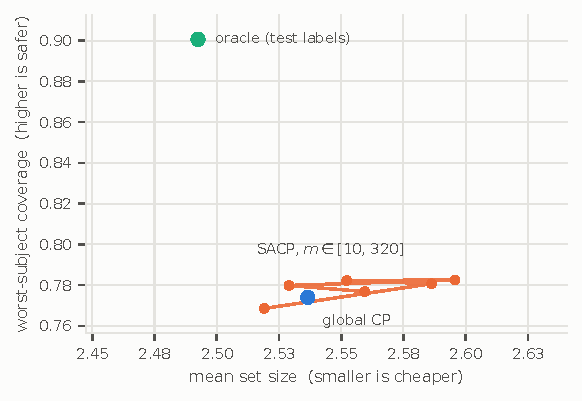
\includegraphics[width=0.72\linewidth]{fig3_pareto.pdf}
  \caption{Worst-patient coverage against mean set size along the warm-up
  budget $m\in\{10,\dots,320\}$, with the shrinkage weight selected by
  leave-one-subject-out simulation at each budget. The blue point is pooled
  calibration, which is also the $m=0$ rule, and the teal point is the oracle
  per-patient threshold computed on the test patient's own labels. The path
  stays next to the pooled point across the whole budget range, and the
  distance to the oracle is what no warm-up rule closes.}
  \label{fig:pareto}
\end{figure}

\begin{table}[t]
\centering
\footnotesize
\setlength{\tabcolsep}{4pt}
\caption{Coverage against the number of calibration subjects $k$, subsampling the available calibration subjects and repeating 50 times per run; rows are averaged over all runs, and $\pm$ is the standard deviation across runs. ``worst'' is the minimum per-subject coverage within a run (each run tests four subjects), averaged over runs, so it is not the merged-cohort worst patient of \Cref{tab:sacp}; it is the quantity that this sweep can hold fixed while $k$ varies. The deficit score's worst-patient coverage is flat in $k$: the patient gap is not calibration-sampling noise.}
\label{tab:cohort-size}
\resizebox{\ifdim\width>\linewidth \linewidth\else\width\fi}{!}{%
\begin{tabular}{rrrrr}
\toprule
\multicolumn{1}{c}{} & \multicolumn{2}{c}{APS} & \multicolumn{2}{c}{Posterior deficit} \\\cmidrule(lr){2-3}\cmidrule(lr){4-5}
$k$ & cov. & worst & cov. & worst \\
\midrule
1 & 0.882\,$\pm$\,0.037 & 0.819\,$\pm$\,0.058 & 0.887\,$\pm$\,0.042 & 0.848\,$\pm$\,0.058 \\
2 & 0.894\,$\pm$\,0.036 & 0.833\,$\pm$\,0.060 & 0.886\,$\pm$\,0.043 & 0.847\,$\pm$\,0.059 \\
3 & 0.896\,$\pm$\,0.038 & 0.837\,$\pm$\,0.062 & 0.889\,$\pm$\,0.044 & 0.850\,$\pm$\,0.060 \\
4 & 0.898\,$\pm$\,0.038 & 0.838\,$\pm$\,0.062 & 0.889\,$\pm$\,0.044 & 0.849\,$\pm$\,0.061 \\
\bottomrule
\end{tabular}}
\par\vspace{2pt}{\footnotesize APS columns are the raw-softmax score; deficit columns use the smoothed posterior deficit. Nominal coverage is 0.900. Calibration pool: 4 subjects.}
\end{table}


\begin{figure}[t]
  \centering
  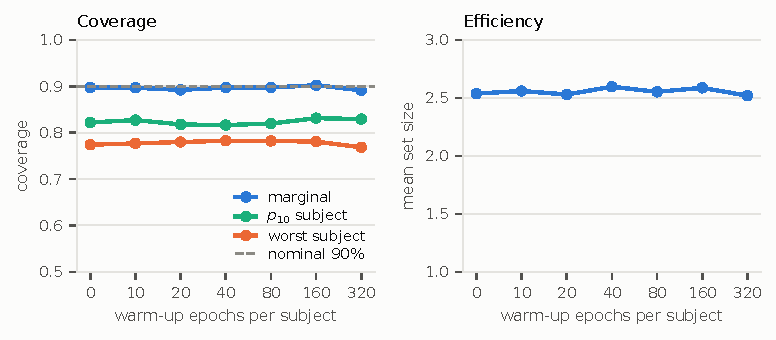
\includegraphics[width=\linewidth]{fig1_budget.pdf}
  \caption{Left: marginal, $p_{10}$ and worst-patient coverage against the
  number of labelled warm-up epochs from the new patient. Right: the
  corresponding mean prediction-set size. The horizontal line marks nominal
  coverage.}
  \label{fig:budget}
\end{figure}

\subsection{Per-patient adaptation collapses the coverage spread}
\label{sec:results-aci}

\Cref{tab:aci} is the central result. Pooled calibration leaves a spread of
$0.051$ across patients and a worst patient at $0.774$. Running one ACI
stream per patient, with the step scale chosen on held-out calibration
streams, collapses the spread to $0.012$ and lifts the worst patient to
$0.886$, at a mean set size of $2.49$ against $2.54$. The deficit score
inherits the correction: its worst patient moves from $0.792$ to $0.872$ at
essentially unchanged set size ($1.53$ to $1.58$), so the efficiency gain of
\Cref{sec:results-score} and the spread collapse of this section compose.

The comparison is paired by patient, and we test the quantity the section is
about rather than the mean. Mean per-patient coverage changes little and not
significantly ($0.896$ to $0.904$, Wilcoxon signed-rank $p=0.84$), but the
distance of a patient's coverage from nominal is smaller under ACI for
$19$ of the $20$ patients (median reduction $0.025$, $p=9.5\times10^{-6}$),
and smaller than under Mondrian for $19$ of $20$ ($p=3.8\times10^{-6}$). The
one patient who moves away from nominal is above it under both rules and
moves by six thousandths (from $0.908$ to $0.914$), well inside the
run-to-run spread. Mondrian is the nearest
alternative on this statistic, and it is not distinguishable from pooled
calibration ($12$ of $20$, $p=0.43$), which is why we read the Mondrian
changes in \Cref{sec:results-patient} as directionally right but not
significant on this cohort.

\Cref{tab:aci-sweep} reports the same experiment at each step scale rather
than at the selected one. The worst patient improves monotonically in
$\gamma_0$ for both scores, from $0.810$ to $0.888$ (APS) and from $0.828$ to
$0.882$ (deficit), and the mean absolute deviation from nominal falls from
$0.030$ to $0.006$ and from $0.026$ to $0.006$. Larger steps are not free: the
fraction of patients below nominal rises from $0.40$ to $0.75$ (APS), because
the recursion pulls every stream toward the marginal rate, and once the spread
has collapsed it is the mean, not the worst patient, that becomes the binding
quantity. The grid stops at $\gamma_0=0.1$ for that reason --- the
spread reduction has saturated while the fraction below nominal is still rising.
The LOSO-selected value ($0.062$ for APS, $0.075$ for the deficit score) sits
below the grid's best row and costs two thousandths of worst-patient coverage
for APS and one point for the deficit score, relative to the best fixed value
in hindsight; that is the price of choosing without the test cohort, and both
are small against the eleven- and eight-point gains over pooled calibration.

One property of \Cref{eq:step} deserves an explicit check. The schedule has
$\sum_t\gamma_t^2=\infty$ and therefore falls outside the
square-summability condition under which the long-run ACI bound is proved, so
the improvement above cannot be attributed to the theory. Repeating the
identical experiment with $\gamma_t=\gamma_0/(t+2)^{0.6}$, which does meet the
condition, leaves the conclusion in place and slightly weaker: worst-patient
coverage $0.877$ against $0.774$ for pooled calibration, per-patient SD
$0.015$ against $0.051$, at a mean set size of $2.51$. The faster-decaying
step adapts more slowly within a night, which is the expected
price of a guarantee that the default schedule does not carry. That guarantee
is \Cref{cor:per-patient}, and it is asymptotic: it says that each patient's
realised miscoverage converges to $\alpha$ as the stream grows, while a night
contributes only a few hundred epochs, so it predicts the direction of the
effect rather than its size. The default schedule is left in the paper
because it is what an implementation would use; the poly-schedule run is
there so that the reader can see the size of the effect under a schedule for
which the corollary actually applies.

\begin{figure}[t]
  \centering
  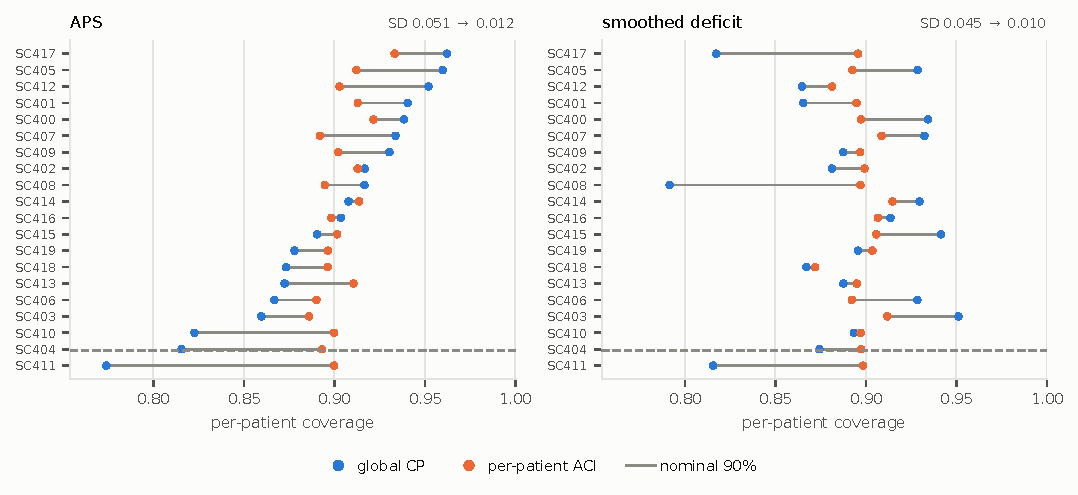
\includegraphics[width=0.9\linewidth]{fig2_subjects.pdf}
  \caption{Per-patient coverage under pooled calibration and under per-patient
  ACI, one line segment per patient, sorted by pooled coverage. Patients to
  the left of the nominal line gain coverage; patients to the right give up
  coverage they did not need.}
  \label{fig:subjects}
\end{figure}

\Cref{fig:subjects} shows the mechanism directly. The reallocation is the
point: the mean coverage is unchanged, and a fraction of patients end up a
hair below nominal by construction, so the fraction-below statistic is not
informative here --- the dispersion and the worst patient are. A single
stream over all patients cannot do this by construction: it returns one
threshold for every patient, so it can move the marginal rate but not the
per-patient dispersion, which is the reason we run one stream per patient.
We therefore do not tabulate a single-stream variant; the comparison that
matters is against the pooled threshold, which is exactly what a single
stream converges to.

\begin{table}[t]
\centering
\small
\setlength{\tabcolsep}{4pt}
\caption{Per-patient adaptive conformal inference at $\alpha=0.1$. Each patient is an independent stream; the step scale is chosen by leave-one-subject-out simulation on the calibration subjects and then applied unchanged to the test cohort.}
\label{tab:aci}
\resizebox{\ifdim\width>\linewidth \linewidth\else\width\fi}{!}{%
\begin{tabular}{lrrrrrrrr}
\toprule
Method & Cov. & Worst & SD & MAD$_\alpha$ & Below & Size & Sing. & Cons. \\
\midrule
Global CP (APS) & 0.898 $\pm$ 0.038 & 0.774 & 0.051 & 0.040 & 0.450 & 2.537 $\pm$ 0.207 & 0.167 $\pm$ 0.051 & 0.680 $\pm$ 0.037 \\
Global CP (deficit) & 0.889 $\pm$ 0.044 & 0.792 & 0.045 & 0.036 & 0.600 & 1.531 $\pm$ 0.325 & 0.841 $\pm$ 0.080 & 0.942 $\pm$ 0.018 \\
Per-patient ACI (APS) & 0.904 $\pm$ 0.010 & 0.886 & 0.012 & 0.009 & 0.500 & 2.491 $\pm$ 0.203 & 0.177 $\pm$ 0.060 & 0.675 $\pm$ 0.020 \\
Per-patient ACI (deficit) & 0.898 $\pm$ 0.007 & 0.872 & 0.010 & 0.007 & 0.700 & 1.575 $\pm$ 0.271 & 0.831 $\pm$ 0.072 & 0.940 $\pm$ 0.014 \\
\bottomrule
\end{tabular}}
\par\vspace{2pt}{\footnotesize Coverage statistics merge per-subject coverage across folds and average each subject over the runs (folds $\times$ seeds $\times$ backbones). Mean LOSO-selected $\gamma_0$ over the runs: aps $= 0.0623$, deficit $= 0.075$. Set size and consistency are averaged over the same runs.}
\end{table}

\begin{table}[t]
\centering
\small
\setlength{\tabcolsep}{4pt}
\caption{Sensitivity of per-patient ACI to the step scale $\gamma_0$ at $\alpha=0.1$. None of these rows is selected on test data; the deployable choice is the LOSO-selected one in \Cref{tab:aci}.}
\label{tab:aci-sweep}
\resizebox{\ifdim\width>\linewidth \linewidth\else\width\fi}{!}{%
\begin{tabular}{lrrrrr}
\toprule
Method & Coverage & Worst subj. & $p_{10}$ subj. & Frac.\ below & Set size \\
\midrule
Per-patient ACI (APS), $\gamma_0=0.005$ & 0.904 $\pm$ 0.026 & 0.810 & 0.864 & 0.400 & 2.566 $\pm$ 0.185 \\
Per-patient ACI (APS), $\gamma_0=0.01$ & 0.908 $\pm$ 0.018 & 0.848 & 0.872 & 0.300 & 2.581 $\pm$ 0.197 \\
Per-patient ACI (APS), $\gamma_0=0.02$ & 0.908 $\pm$ 0.011 & 0.875 & 0.887 & 0.400 & 2.553 $\pm$ 0.199 \\
Per-patient ACI (APS), $\gamma_0=0.05$ & 0.902 $\pm$ 0.006 & 0.885 & 0.891 & 0.500 & 2.469 $\pm$ 0.177 \\
Per-patient ACI (APS), $\gamma_0=0.1$ & 0.898 $\pm$ 0.004 & 0.888 & 0.890 & 0.750 & 2.409 $\pm$ 0.163 \\
Per-patient ACI (deficit), $\gamma_0=0.005$ & 0.894 $\pm$ 0.030 & 0.828 & 0.859 & 0.600 & 1.579 $\pm$ 0.255 \\
Per-patient ACI (deficit), $\gamma_0=0.01$ & 0.898 $\pm$ 0.021 & 0.859 & 0.862 & 0.600 & 1.613 $\pm$ 0.260 \\
Per-patient ACI (deficit), $\gamma_0=0.02$ & 0.900 $\pm$ 0.014 & 0.860 & 0.884 & 0.600 & 1.616 $\pm$ 0.268 \\
Per-patient ACI (deficit), $\gamma_0=0.05$ & 0.899 $\pm$ 0.007 & 0.873 & 0.887 & 0.550 & 1.590 $\pm$ 0.267 \\
Per-patient ACI (deficit), $\gamma_0=0.1$ & 0.898 $\pm$ 0.004 & 0.882 & 0.889 & 0.650 & 1.562 $\pm$ 0.265 \\
\bottomrule
\end{tabular}}
\end{table}


\subsection{Sequence constructors: a negative result}
\label{sec:results-temporal}

\Cref{tab:temporal} reports the dynamic-programming constructors alongside
their per-epoch comparators. The first block uses every test epoch and
includes the per-stage deficit threshold of \Cref{sec:results-score}, so that
the score-family comparison is in one place; the constructor blocks use only
the epochs inside complete blocks, and the per-epoch baseline immediately
above the SeqCP-Margin block is recalibrated on exactly those epochs. Three
observations follow, and they are the reason we do not present these
constructors as a contribution.

\emph{At $\beta=0$ the margin constructor is exactly per-epoch split CP} on the
deficit score (Proposition~\ref{prop:reduction}). The numerical check in the
test suite confirms the identity to machine precision, and
\Cref{tab:temporal} confirms it at the level of realised coverage and set
size: the $\beta=0$ row and the baseline above it agree to every reported
digit. This is not a nuisance: it is what allows the $\beta>0$ rows to be
interpreted as the effect of the transition term alone.

\emph{At $\beta>0$ the sets get larger.} The block-level set is a union over
admissible sequences, and the transition penalty makes low-transition
sequences cheap; at $\beta\ge0.5$ a constant sequence is admissible for every
label, the projection is the whole label set, and sequence coverage is
$1.000$ by triviality. The simultaneous guarantee of
Theorem~\ref{thm:projection} holds and is vacuous. \Cref{tab:temporal}'s
SeqCP-Block rows show this directly.

\emph{The transition structure is already in the score.} The smoothed
posterior that the deficit score is computed from has absorbed the same
Markov structure that the dynamic program is meant to exploit. Re-imposing it
at the level of the set adds looseness rather than information. This is why
the efficiency gain in \Cref{sec:results-score} comes from smoothing, not
from sequence construction, and it is the substantive lesson of the
ablation.

\Cref{fig:hypnogram} shows the consequence on a real recording: pooled APS
produces sets that flicker at transitions, the deficit score produces stable
singleton sets through stable stretches and wider sets at transitions, and
per-patient ACI widens the sets for a patient whose pooled coverage was low.

\begin{figure}[t]
  \centering
  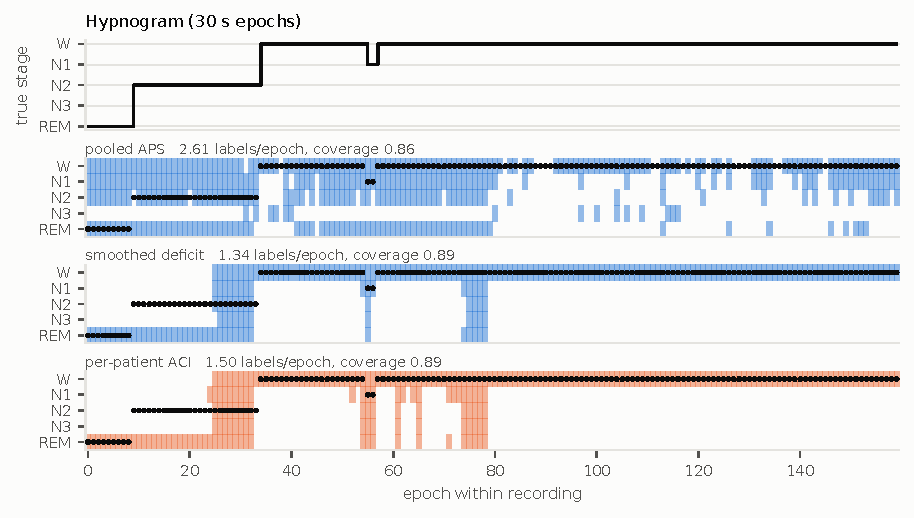
\includegraphics[width=\linewidth]{fig4_hypnogram.pdf}
  \caption{A \num{160}-epoch window of one test recording (subject SC409),
  chosen because it spans a stage transition. Top: the scored hypnogram.
  Panels: one row per stage, with a shaded cell where that stage is in the
  prediction set under pooled APS, smoothed deficit, and per-patient ACI. The
  black dots repeat the true stage inside each panel, so an epoch is covered
  exactly when its dot lies on a shaded cell; the label count and coverage
  printed with each panel are over this window only.}
  \label{fig:hypnogram}
\end{figure}

\begin{table}[t]
\centering
\small
\setlength{\tabcolsep}{4pt}
\caption{Temporal conformal prediction at $\alpha=0.1$, block length $L=10$. The first four rows use every test epoch; the rows below them use only the epochs inside complete blocks, and the per-epoch baseline above the SeqCP-Margin block is recalibrated on exactly those epochs.}
\label{tab:temporal}
\resizebox{\ifdim\width>\linewidth \linewidth\else\width\fi}{!}{%
\begin{tabular}{lrrrrrr}
\toprule
Method & Coverage & Set size & Singleton & Review & Consistency & Seq.\ coverage \\
\midrule
Smoothed deficit (all epochs) & 0.889 $\pm$ 0.044 & 1.531 $\pm$ 0.325 & 0.841 $\pm$ 0.080 & 0.159 $\pm$ 0.080 & 0.942 $\pm$ 0.018 & -- \\
Smoothed deficit, per stage & 0.903 $\pm$ 0.034 & 1.741 $\pm$ 0.252 & 0.506 $\pm$ 0.104 & 0.494 $\pm$ 0.104 & 0.884 $\pm$ 0.016 & -- \\
Smoothed APS (all epochs) & 0.903 $\pm$ 0.037 & 2.223 $\pm$ 0.170 & 0.229 $\pm$ 0.053 & 0.712 $\pm$ 0.062 & 0.753 $\pm$ 0.036 & -- \\
Per-epoch APS (all epochs) & 0.898 $\pm$ 0.038 & 2.537 $\pm$ 0.207 & 0.167 $\pm$ 0.051 & 0.765 $\pm$ 0.060 & 0.680 $\pm$ 0.037 & -- \\
\addlinespace[3pt]
Smoothed deficit, $L=10$ epochs & 0.889 $\pm$ 0.045 & 1.535 $\pm$ 0.326 & 0.840 $\pm$ 0.080 & 0.160 $\pm$ 0.080 & 0.942 $\pm$ 0.018 & -- \\
SeqCP-Margin L10, $\beta=0$ & 0.889 $\pm$ 0.045 & 1.535 $\pm$ 0.326 & 0.840 $\pm$ 0.080 & 0.160 $\pm$ 0.080 & 0.942 $\pm$ 0.018 & 0.668 $\pm$ 0.089 \\
SeqCP-Margin L10, $\beta=0.5$ & 0.890 $\pm$ 0.045 & 1.941 $\pm$ 0.616 & 0.688 $\pm$ 0.215 & 0.312 $\pm$ 0.215 & 0.865 $\pm$ 0.061 & 0.682 $\pm$ 0.096 \\
SeqCP-Margin L10, $\beta=1$ & 0.891 $\pm$ 0.045 & 1.993 $\pm$ 0.634 & 0.655 $\pm$ 0.230 & 0.345 $\pm$ 0.230 & 0.864 $\pm$ 0.060 & 0.688 $\pm$ 0.096 \\
SeqCP-Margin L10, $\beta=2$ & 0.889 $\pm$ 0.045 & 2.016 $\pm$ 0.625 & 0.666 $\pm$ 0.166 & 0.334 $\pm$ 0.166 & 0.863 $\pm$ 0.062 & 0.680 $\pm$ 0.080 \\
\addlinespace[3pt]
SeqCP-Block L10, $\beta=0$ & 0.919 $\pm$ 0.032 & 4.570 $\pm$ 0.167 & 0.005 $\pm$ 0.002 & 0.914 $\pm$ 0.033 & 0.909 $\pm$ 0.035 & 0.917 $\pm$ 0.033 \\
SeqCP-Block L10, $\beta\ge0.5$ & 1.000 $\pm$ 0.000 & 5.000 $\pm$ 0.000 & 0.000 $\pm$ 0.000 & 1.000 $\pm$ 0.000 & 1.000 $\pm$ 0.000 & 1.000 $\pm$ 0.000 \\
\bottomrule
\end{tabular}}
\par\vspace{2pt}{\footnotesize ``Review'' is the fraction of epochs whose set contains more than one stage and would need adjudication; ``Consistency'' is the mean Jaccard overlap of adjacent prediction sets within a recording; ``Seq.\ coverage'' is the fraction of blocks whose every epoch is covered. The SeqCP-Block rows at $\beta=0.5,1,2$ coincide exactly; $L=20$ and $L=30$ change no conclusion; the full sweep is in the released JSON. SeqCP-Margin at $\beta=0$ coincides with the per-epoch baseline of the same name to every reported digit, which is the numerical check of \Cref{prop:reduction}; realised coverage is an expectation over calibration draws, not a bound for a single calibration set.}
\end{table}


\subsection{Robustness to hardware shift and input corruption}
\label{sec:results-shift}

\Cref{tab:shift} reports coverage under hardware shift: the model is trained
on one Sleep-EDF cohort (cassette or telemetry), calibrated on four held-out
subjects of that cohort, and tested on the other. The ranking of scores
changes. The deficit score, the most efficient in-cohort, is also the most
fragile: pooled coverage falls from $0.889$ to $0.835$ (cassette to telemetry)
and $0.878$ (telemetry to cassette), and the worst patient falls to $0.714$
and $0.678$. Two mechanisms contribute --- the forward--backward pass uses
transition matrices estimated from source-cohort labels, and the posterior
sharpness changes with the signal statistics of the target cohort. Pooled APS
holds coverage better --- it over-covers at $0.933$ in one direction and sits
at $0.886$ in the other --- but its worst patient is at $0.799$ and $0.789$,
and it pays with the largest sets ($2.68$ and $2.20$ labels per epoch).
Per-patient ACI, which adapts on the target stream and therefore does not
assume the calibration cohort matches the target population, brings marginal
coverage back to between $0.896$ and $0.913$ in both directions and lifts the
worst patient to $0.883$ and $0.872$ for APS and to $0.878$ in both
directions for the deficit score; for the deficit score this costs $32\%$ and
$6\%$ in mean set size ($1.40\to1.84$ and $1.77\to1.87$).

\Cref{tab:corruption} applies controlled corruptions to the test signals while
calibration stays clean, and contrasts three thresholds: the clean one, one
refitted on identically corrupted calibration signals, and one adapted online
by per-patient ACI. The loss is not monotone in severity across corruption
families, and it is not always a loss: a circular time shift, which preserves
the spectrum, moves coverage by less than a thousandth and leaves accuracy
unchanged, and zeroing a fifth of the epochs costs $1.3$ points of
coverage for twelve points of accuracy. Where the corruption bites, the clean
threshold fails catastrophically ($0.497$ coverage at $0\,\mathrm{dB}$ SNR,
$0.141$ under $2\sigma$ baseline drift), and both adaptations restore
coverage ($0.892$ and $0.929$ by recalibration; $0.893$ and $0.890$ by ACI).
Recalibration restores more than the number: corrupted calibration and
corrupted test signals are exchangeable again, so the split-conformal
guarantee applies to the corrupted data. ACI makes no such argument --- it
carries the long-run property of \Cref{sec:method-aci} --- and its values
here are measured, not proved.

The accuracy column is the reason to read that recovery carefully. Under the
same two corruptions the classifier itself is at $0.257$ and $0.252$, against
$0.802$ clean. What the recalibrated threshold restores is the truthfulness of
the set, not the model, and it pays for the truth by reporting larger sets
($3.44$ and $3.93$ labels per epoch against $3.00$ clean). ACI, which never
sees corrupted calibration data, reaches the same coverage at $3.30$ and
$3.32$. A deployment that reports only coverage would call this a recovery;
one that reports coverage and set size sees a model that has stopped working
and a predictor that says so --- which is the behaviour we want, provided the
set size is reported.

\begin{table}[t]
\centering
\footnotesize
\setlength{\tabcolsep}{4pt}
\caption{Coverage under hardware shift. The in-cohort rows are the cassette cohort over all runs of the main matrix; the cross rows train on one cohort, calibrate on four held-out subjects from it, and test on the other cohort, at seed 0 for both backbones, with the statistics merged over the five folds and two backbones. The $\pm$ is the standard deviation over the runs contributing to the row (thirty in-cohort, ten cross-cohort), so it measures run-to-run variation, not uncertainty over patients. Per-patient ACI uses the leave-one-subject-out step size selected within the source cohort.}
\label{tab:shift}
\resizebox{\ifdim\width>\linewidth \linewidth\else\width\fi}{!}{%
\begin{tabular}{llrrrr}
\toprule
Scenario & Method & Coverage & Worst patient & $p_{10}$ & Set size \\
\midrule
In-cohort & APS, pooled & 0.898 $\pm$ 0.038 & 0.774 & 0.822 & 2.537 $\pm$ 0.207 \\
 & APS, per-patient ACI & 0.904 $\pm$ 0.010 & 0.886 & 0.892 & 2.491 $\pm$ 0.203 \\
 & Deficit, pooled & 0.889 $\pm$ 0.044 & 0.792 & 0.817 & 1.531 $\pm$ 0.325 \\
 & Deficit, per-patient ACI & 0.898 $\pm$ 0.007 & 0.872 & 0.891 & 1.575 $\pm$ 0.271 \\
\addlinespace[2pt]
Cassette $\to$ telemetry & APS, pooled & 0.933 $\pm$ 0.028 & 0.799 & 0.869 & 2.684 $\pm$ 0.066 \\
 & APS, per-patient ACI & 0.913 $\pm$ 0.010 & 0.883 & 0.894 & 2.387 $\pm$ 0.018 \\
 & Deficit, pooled & 0.835 $\pm$ 0.026 & 0.714 & 0.747 & 1.397 $\pm$ 0.083 \\
 & Deficit, per-patient ACI & 0.896 $\pm$ 0.001 & 0.878 & 0.888 & 1.843 $\pm$ 0.099 \\
\addlinespace[2pt]
Telemetry $\to$ cassette & APS, pooled & 0.886 $\pm$ 0.003 & 0.789 & 0.838 & 2.198 $\pm$ 0.079 \\
 & APS, per-patient ACI & 0.903 $\pm$ 0.001 & 0.872 & 0.883 & 2.292 $\pm$ 0.152 \\
 & Deficit, pooled & 0.878 $\pm$ 0.001 & 0.678 & 0.820 & 1.772 $\pm$ 0.280 \\
 & Deficit, per-patient ACI & 0.898 $\pm$ 0.005 & 0.878 & 0.880 & 1.874 $\pm$ 0.264 \\
\bottomrule
\end{tabular}}
\end{table}

\begin{table}[t]
\centering
\footnotesize
\setlength{\tabcolsep}{4pt}
\caption{Coverage at the most severe level of each input corruption, applied to the test signals only. Accuracy is the corrupted model's own epoch accuracy and does not depend on any threshold. ``Clean threshold'' is the split-conformal threshold fitted on clean calibration data; ``recalibrated'' refits the threshold on calibration signals corrupted identically, and the following column is the mean set size it returns; ``per-patient ACI'' adapts the threshold online on the corrupted stream using the clean calibration set, again with its mean set size. One representative run (EEGNet, fold 0) is reported because the corruption is a property of the model and the split rather than of the fold.}
\label{tab:corruption}
\resizebox{\ifdim\width>\linewidth \linewidth\else\width\fi}{!}{%
\begin{tabular}{llrrrrrr}
\toprule
Corruption & Severity & Accuracy & Clean threshold & Recalibrated & Recal.\ size & Per-patient ACI & ACI size \\
\midrule
None & -- & 0.802 & 0.936 & 0.936 & 3.00 & 0.936 & 3.00 \\
Noise & 0 dB SNR & 0.257 & 0.497 & 0.892 & 3.44 & 0.893 & 3.30 \\
Amplitude scale & $\times 1.5$ & 0.717 & 0.831 & 0.964 & 2.90 & 0.896 & 2.38 \\
Baseline drift & $2\sigma$ wander & 0.252 & 0.141 & 0.929 & 3.93 & 0.890 & 3.32 \\
Circular time shift & 5 s & 0.802 & 0.936 & 0.937 & 3.00 & 0.902 & 2.65 \\
Epoch dropout & 20\% & 0.683 & 0.923 & 0.921 & 3.17 & 0.902 & 3.06 \\
\bottomrule
\end{tabular}}
\end{table}


\subsection{Extended cohort}
\label{sec:results-cohort}

The 78-subject cohort increases the number of test subjects per fold from four
to fifteen or sixteen (and the calibration cohort from four to sixteen), and
lets the worst-patient statistics be estimated with
less noise. \Cref{tab:extended} reports the same headline comparison; the
ordering of methods is unchanged and the pooled-to-per-patient gap is larger,
from $0.641$ to $0.879$ (APS) against $0.774$ to $0.886$ in the 20-subject
cohort. Part of that widening is mechanical, since the minimum is taken over
nearly four times as many patients, but the per-patient SD says the same
thing without an extremum: $0.067$ against $0.016$ for APS and $0.053$
against $0.013$ for the deficit score, both larger than the corresponding
$0.051$ and $0.045$ against $0.012$ and $0.010$ of \Cref{tab:aci}.

\begin{table}[t]
\centering
\small
\setlength{\tabcolsep}{4pt}
\caption{The headline comparison of \Cref{tab:sacp} repeated on the 78-subject cohort, at seed 0. Test blocks of fifteen or sixteen subjects make each fold's estimate less sensitive to a single night, while the minimum over all subjects is naturally more extreme than in the smaller cohort.}
\label{tab:extended}
\resizebox{\ifdim\width>\linewidth \linewidth\else\width\fi}{!}{%
\begin{tabular}{lrrrrrrr}
\toprule
Method & Coverage & Worst subj. & $p_{10}$ subj. & SD & Below & Set size & Singleton \\
\midrule
Random-epoch split & 0.900 & -- & -- & -- & -- & 2.898 & -- \\
Pooled (APS) & 0.898 $\pm$ 0.036 & 0.641 & 0.822 & 0.0667 & 0.33 & 2.890 $\pm$ 0.231 & 0.059 $\pm$ 0.031 \\
Pooled (RAPS) & 0.905 $\pm$ 0.031 & 0.751 & 0.854 & 0.0380 & 0.37 & 1.845 $\pm$ 0.271 & 0.306 $\pm$ 0.204 \\
Mondrian (per class) & 0.908 $\pm$ 0.030 & 0.681 & 0.840 & 0.0599 & 0.33 & 2.306 $\pm$ 0.111 & 0.261 $\pm$ 0.030 \\
$k$NN subject (APS) & 0.893 $\pm$ 0.032 & 0.678 & 0.843 & 0.0627 & 0.42 & 2.776 $\pm$ 0.170 & 0.072 $\pm$ 0.029 \\
Warm-up SACP, $m=80$ & 0.915 $\pm$ 0.043 & 0.631 & 0.840 & 0.0704 & 0.24 & 3.075 $\pm$ 0.414 & 0.073 $\pm$ 0.031 \\
Warm-up SACP, $m=320$ & 0.898 $\pm$ 0.029 & 0.700 & 0.852 & 0.0481 & 0.38 & 2.847 $\pm$ 0.308 & 0.078 $\pm$ 0.031 \\
Oracle per patient & 0.906 $\pm$ 0.011 & 0.900 & 0.901 & 0.0137 & 0.00 & 2.758 $\pm$ 0.181 & 0.094 $\pm$ 0.025 \\
Per-patient ACI (APS) & 0.917 $\pm$ 0.007 & 0.879 & 0.898 & 0.0163 & 0.14 & 2.898 $\pm$ 0.152 & 0.072 $\pm$ 0.028 \\
Per-patient ACI (deficit) & 0.897 $\pm$ 0.004 & 0.861 & 0.884 & 0.0133 & 0.54 & 1.657 $\pm$ 0.157 & 0.805 $\pm$ 0.045 \\
\bottomrule
\end{tabular}}
\par\vspace{2pt}{\footnotesize ``Coverage'' is marginal over epochs (mean $\pm$ SD over the runs); ``Worst subj.'' is the minimum per-subject coverage over the runs; ``Below'' is the fraction of subjects below $1-\alpha$; ``SD'' is the standard deviation of per-subject coverage. Each subject contributes one value per run, the runs being five folds $\times$ one seed $\times$ two backbones; set size and singleton rate are averaged over the same runs.}
\end{table}

